\documentclass[twoside]{article}
\usepackage{ecj,palatino,epsfig,latexsym,natbib}
\usepackage{graphicx,caption,subcaption}

%% do not add any other page- or text-size instruction here

\parskip=0.00in

\begin{document}

\ecjHeader{x}{x}{xxx-xxx}{201X}{45-character paper description goes here}{Author(s) initials and last name go here}
\title{\bf Using Neural Networks to produce Mutation Distributions}  

\author{\name{\bf Alexander W. Churchill} \hfill \addr{alexanderchurchill@gmail.com}\\ 
        \addr{Queen Mary, University of London}
\AND
       \name{\bf Siddarth Sigtia} \hfill \addr{author2@abc.university.country}\\
        \addr{Queen Mary, University of London}
\AND
       \name{\bf Chrisantha Fernando} \hfill \addr{author2@abc.university.country}\\
        \addr{Queen Mary, University of London}
}

\maketitle

\begin{abstract}

Neural networks and evolutionary computation have a rich intertwined history. They most commonly appear together when an evolutionary algorithm is used to optimise the parameters and topology of a neural network for reinforcement learning problems or for supervised learning when complex temporal dynamics are required. In this paper we take the opposite approach, asking the question of whether a neural network can be used to provide a mutation distribution for an evolutionary algorithm, and what advantages this approach may offer? 

\end{abstract}

\begin{keywords}

Genetic algorithms, 
Estimation of Distribution algorithms,
Autoencoder,
Neural Autoregressive Distribution Estimator,
Neural Networks.

\end{keywords}
\section{Results}
Figures \ref{figure:results_plots1} and \ref{figure:results_plots2} show for different test problems plots of the best found fitness as the number of evaluations increase, averaged across ten independent trials, as well as boxplots showing the distribution of the best found solutions at the end of the optimisation process. Results are also summarised in table \ref{table_results}. We observe that on four of the six problems, either GA-dA or GA-NADE performs the best, with BOA outperforming both on the two HIFF problems.

On the MaxSat problem GA-NADE is the only algorithm that reaches the optimum on all 10 trials. Although both GA-NADE and GA-dA progress in a similar manner earlier in the search process, GA-NADE continues to improve and finds the optimal solution of 430 much more quickly, within around 140,000 evaluations. Interestingly BOA is unable to find the optimal solution within the evaluation limit, although it performs much better than PBIL and the GA on average.

GA-dA is by far the best performer on both knapsack problems. On the 500-item instance it is the only algorithm that locates the optimal solution and on the Weing8 instance with two constraints it has a much greater success rate than the next best. On both problems it also improves much more quickly than the other algorithms. Both GA-NADE and BOA have much slower rates of improvement than GA-dA, although GA-NADE is considerably faster than BOA. BOA finds slightly better solutions than GA-NADE on the 500-item knapsack but performs considerably worse on the Weing8 instance.

On both tested HIFF instances BOA is the far greater performer, solving the 128-bit problem twice as fast and the 256-bit instance three times faster than GA-NADE. In turn, GA-NADE is able to solve the 128-bit instance in half the evaluations required from GA-dA and a quarter as many on the 256-bit instance. GA-dA is better than the standard GA on this problem, solving it faster and more consistently. The GA is not able to solve the HIFF instances on every trial, although it can locate the optimal solution while PBIL cannot.

GA-dA displays the best performance on the Royal Road problem, consistently solving it within a small number of evaluations. The next best is the GA which can solve it more quickly but has much greater variance in discovery times. BOA is able to solve the problem much faster on average than GA-NADE, with low variance in terms of the number of evaluations taken to solve the problem. 
\begin{figure}[t!]
\centering
    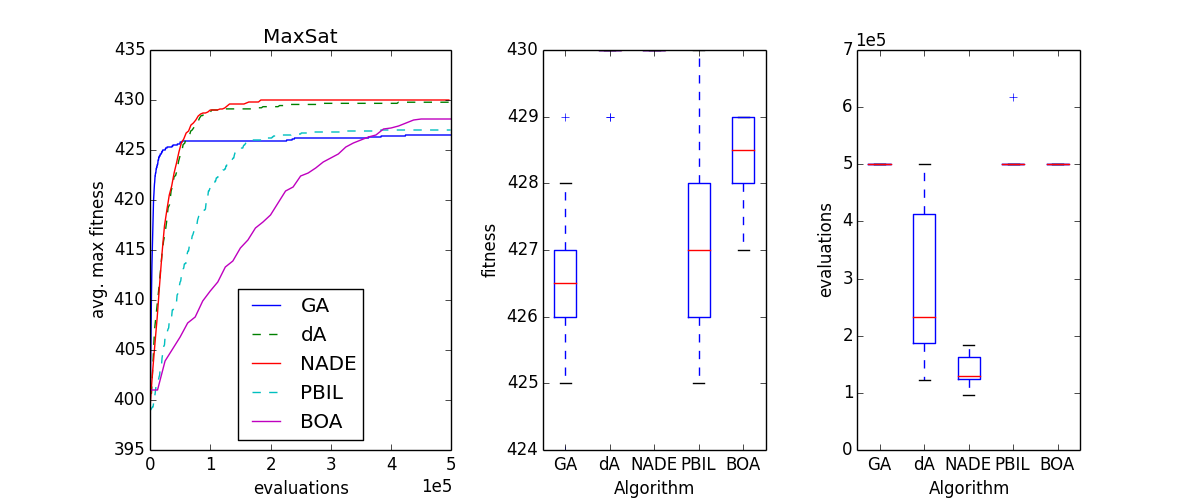
\includegraphics[scale=0.38]{results/maxsat.png}
    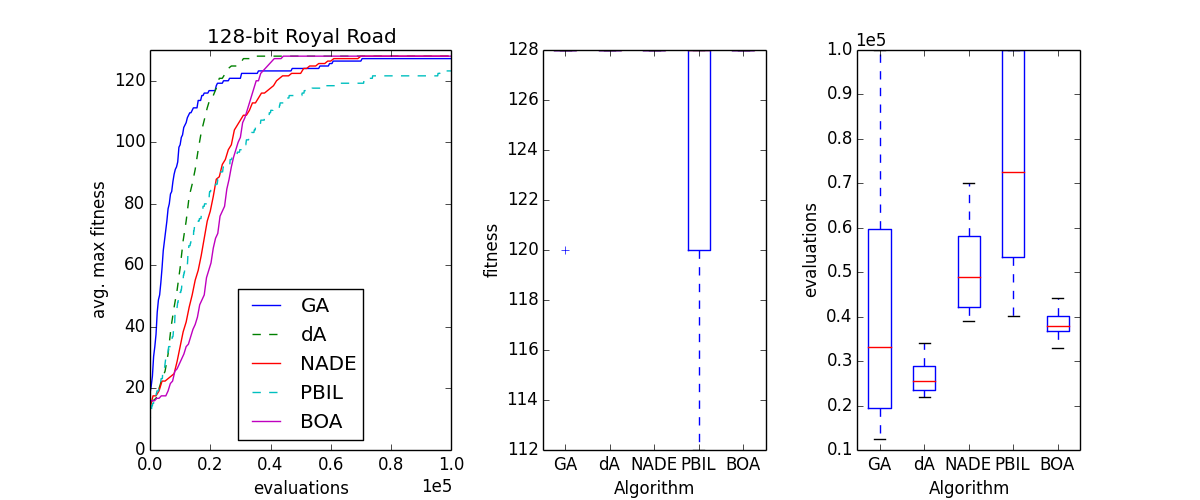
\includegraphics[scale=0.38]{results/royal_road.png}
    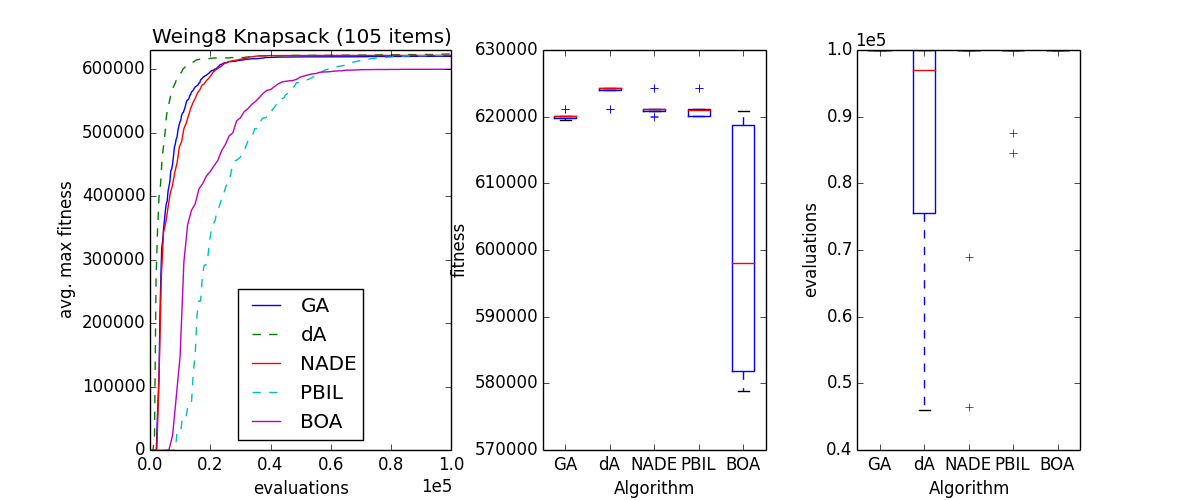
\includegraphics[scale=0.38]{results/knapsack_105.png}
    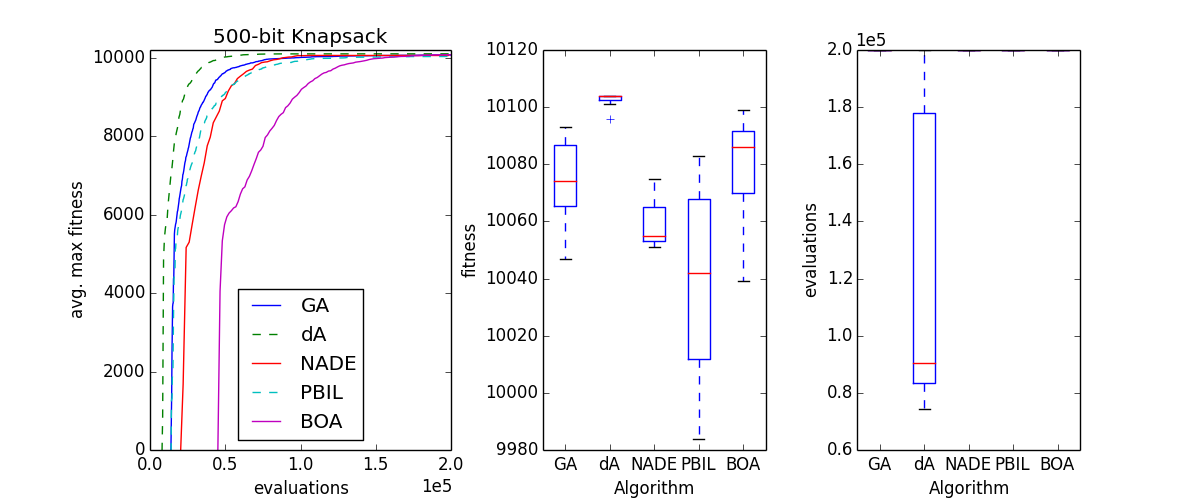
\includegraphics[scale=0.38]{results/knapsack_500.png}
  \caption{}
  \label{figure:results_plots1}
\end{figure}
\begin{figure}[t!]
\centering
  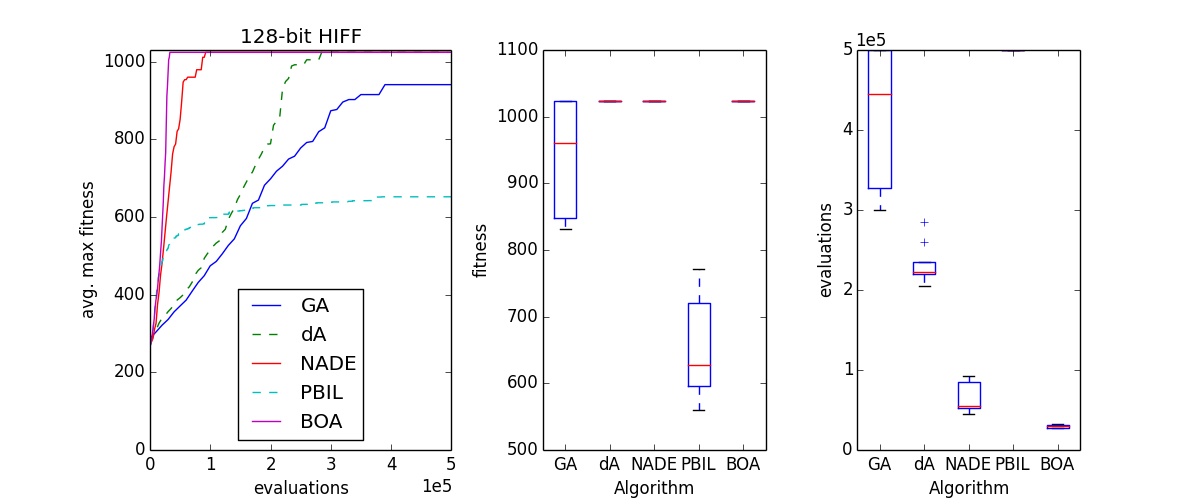
\includegraphics[scale=0.38]{results/hiff128.png}
    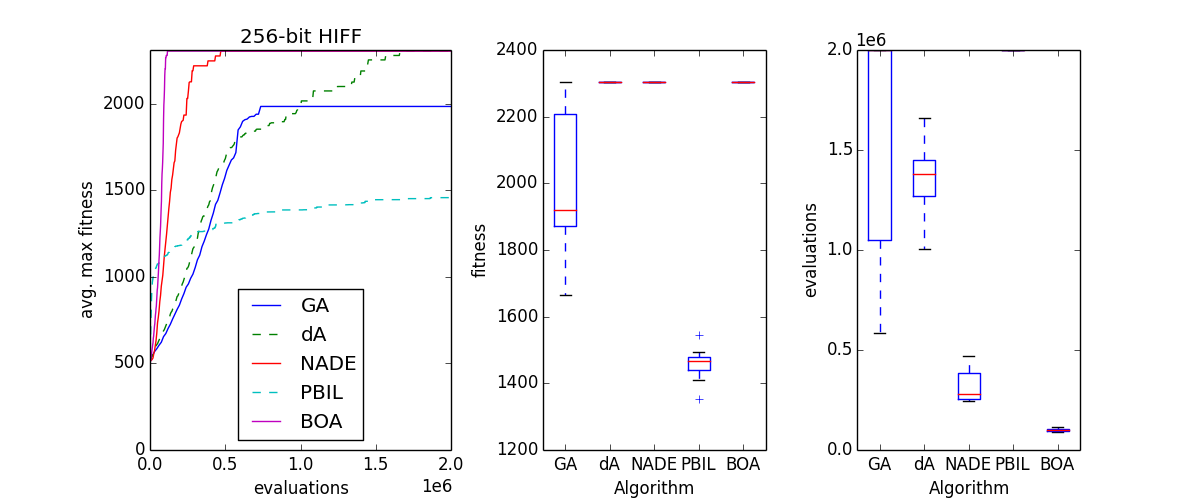
\includegraphics[scale=0.38]{results/hiff256.png}
  \caption{}
    \label{figure:results_plots2}
\end{figure}

 \begin{table}[t!]
   \scalebox{0.8}{
    \begin{tabular}{ | p{1.8cm} | l | l | l | l | l | l | l | l | p{1cm} |}
    \hline
    Experiment & Algorithm & Min & Max & Mean & Mean Evals & Success \%\\ \hline
Royal Road 128 & GA & 120.0 & 128.0 & 127.20 \(\pm\)2 & 42600.00 \(\pm\)27034 & 90\%\\
 & dA & 128.0 & 128.0 & 128.00 \(\pm\)0 & 26500.00 \(\pm\)3721 & 100\%\\
 & NADE & 128.0 & 128.0 & 128.00 \(\pm\)0 & 50900.00 \(\pm\)9771 & 100\%\\
 & PBIL & 112.0 & 128.0 & 123.20 \(\pm\)6 & 74110.00 \(\pm\)23463 & 60\%\\
 & BOA & 128.0 & 128.0 & 128.00 \(\pm\)0 & 38175.00 \(\pm\)3118 & 100\%\\\hline
MaxSat & GA & 424.0 & 429.0 & 426.50 \(\pm\)1 & 500000.00 \(\pm\)0 & 0\%\\
 & dA & 429.0 & 430.0 & 429.78 \(\pm\)0 & 291944.44 \(\pm\)134967 & 70\%\\
 & NADE & 430.0 & 430.0 & 430.00 \(\pm\)0 & 141600.00 \(\pm\)28182 & 100\%\\
 & PBIL & 425.0 & 430.0 & 427.10 \(\pm\)1 & 511800.00 \(\pm\)35400 & 10\%\\
 & BOA & 427.0 & 429.0 & 428.30 \(\pm\)0 & 500000.00 \(\pm\)0 & 0\%\\\hline
HIFF 128 & GA & 832.0 & 1024.0 & 940.80 \(\pm\)86 & 416000.00 \(\pm\)87429 & 50\%\\
 & dA & 1024.0 & 1024.0 & 1024.00 \(\pm\)0 & 231000.00 \(\pm\)23537 & 100\%\\
 & NADE & 1024.0 & 1024.0 & 1024.00 \(\pm\)0 & 65500.00 \(\pm\)17492 & 100\%\\
 & PBIL & 560.0 & 772.0 & 652.00 \(\pm\)76 & 500000.00 \(\pm\)0 & 0\%\\
 & BOA & 1024.0 & 1024.0 & 1024.00 \(\pm\)0 & 29400.00 \(\pm\)1854 & 100\%\\\hline
HIFF 256 & GA & 1664.0 & 2304.0 & 1984.00 \(\pm\)225 & 1590500.00 \(\pm\)626719 & 30\%\\
 & dA & 2304.0 & 2304.0 & 2304.00 \(\pm\)0 & 1355500.00 \(\pm\)190793 & 100\%\\
 & NADE & 2304.0 & 2304.0 & 2304.00 \(\pm\)0 & 318333.33 \(\pm\)82663 & 90\%\\
 & PBIL & 1354.0 & 1544.0 & 1457.40 \(\pm\)48 & 2000000.00 \(\pm\)0 & 0\%\\
 & BOA & 2304.0 & 2304.0 & 2304.00 \(\pm\)0 & 98800.00 \(\pm\)7493 & 100\%\\\hline
Knapsack 500 & GA & 10047.0 & 10093.0 & 10074.20 \(\pm\)13 & 200000.00 \(\pm\)0 & 0\%\\
 & dA & 10096.0 & 10104.0 & 10102.70 \(\pm\)2 & 121620.00 \(\pm\)52114 & 70\%\\
 & NADE & 10051.0 & 10075.0 & 10060.33 \(\pm\)10 & 200000.00 \(\pm\)0 & 0\%\\
 & PBIL & 9984.0 & 10083.0 & 10039.00 \(\pm\)31 & 200000.00 \(\pm\)0 & 0\%\\
 & BOA & 10039.0 & 10099.0 & 10079.40 \(\pm\)17 & 200000.00 \(\pm\)0 & 0\%\\\hline
Weing8 Knapsack & GA & 619568.0 & 621086.0 & 620137.40 \(\pm\)511 & 100000.00 \(\pm\)0 & 0\%\\
 & dA & 621086.0 & 624319.0 & 623615.40 \(\pm\)1270 & 85400.00 \(\pm\)19172 & 60\%\\
 & NADE & 619886.0 & 624319.0 & 621483.50 \(\pm\)1479 & 91550.00 \(\pm\)17632 & 20\%\\
 & PBIL & 620060.0 & 624319.0 & 621304.80 \(\pm\)1566 & 97220.00 \(\pm\)5600 & 20\%\\
 & BOA & 578923.0 & 620821.0 & 599630.20 \(\pm\)17700 & 100000.00 \(\pm\)0 & 0\%\\\hline
    \end{tabular}
    }
    \caption{Results for DAGA and the GA on 6 discrete problems. Showing the value of the minimum and maximum solution returned at the end of search, the mean best solution in the population after the end of search, the mean number of evaluations required to reach the optimum solution (or until the maximum number of evaluations) and the success rate for reaching the optimum, averaged across 10 trials. Stars indicate that the mean result for the specified algorithm is significantly different from the GA according to a Wilcoxan Rank Sum test (\(p<0.05\)).}
        \label{table:main_results}

\end{table}


\section{Discussion}

The results described in the preceding section show that the Autoencoder (GA-dA) and NADE (GA-NADE) methods perform well across a number of different problems. GA-dA significantly outperforms the other methods on both knapsack problems and the Royal Road. GA-NADE is the only algorithm that is able to solve the MaxSat problem consistently. There are clear differences in the performance of the two Neural Network based algorithms, with GA-NADE performing much better on the HIFF and MaxSat problems but significantly worse on the others. The two methods discover structure in solution space in considerably different ways, with GA-NADE creating a generative model in the form of a Bayesian graph and GA-dA through a compressed encoding of promising solutions. To investigate the differences between the two models, a new objective function has been devised based on Mitchell's Royal Road [\cite{mitchell}].
\begin{figure}[t!]
\centering
    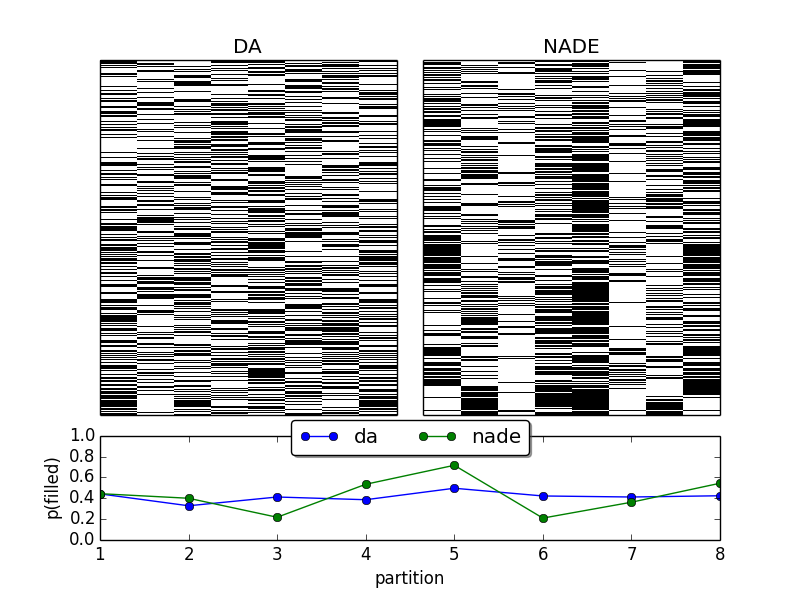
\includegraphics[scale=0.6]{nade-vs-da-wide.png}
  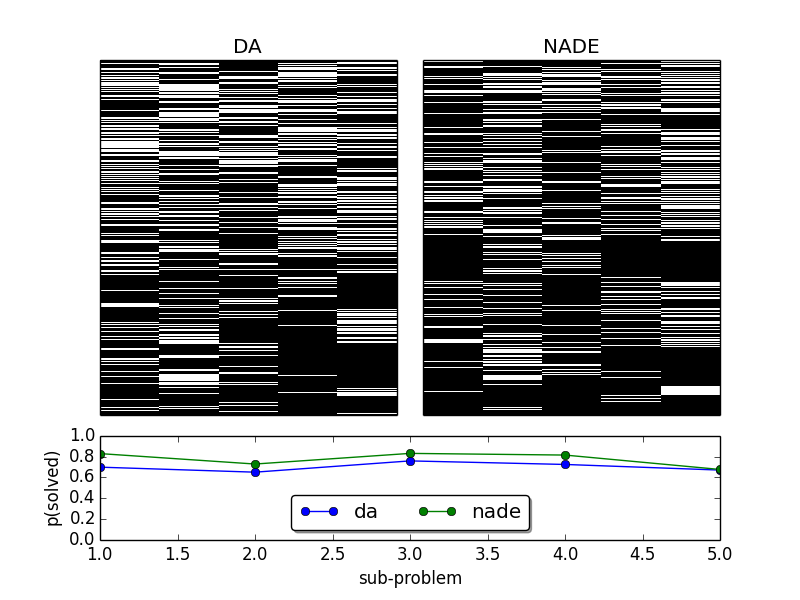
\includegraphics[scale=0.6]{nade-vs-da-narrow.png}
  \caption{}
\end{figure}

For a given bit string consists of \(x\) non-overlapping partitions, \(p\), of size \(2k\), each partition, \(p_i\), is further divided into two non-overlapping partitions of size \(k\), \(\hat{p}_{iL}\) on the left side and \(\hat{p}_{iR}\) on the right. If each bit in \(\hat{p}_{iL}\) is equal to 1 and each bit in \(\hat{p}_{iR}\) is equal to 0, 1 is added to fitness. Alternatively, a 1 is added to fitness if each bit in \(\hat{p}_{iL}\) is equal to 0 and each bit in \(\hat{p}_{iR}\) is equal to 1. Finally, an additional 1 is added to fitness if every bit in \(\hat{p}_{1L}\) and \(\hat{p}_{xR}\) are equal to 1, or if every bit in \(\hat{p}_{1L}\) and \(\hat{p}_{xR}\) is equal to 0, where \(i=1\) signifies the first partition and \(i=x\) the last. An example is given for a 16-bit sequence in fig. . This fitness function has been invented to explore how the algorithms deal with dependency between blocks of variables.

GA-NADE and GA-dA were applied to a 32-bit version of this problem, both using a population size of 500. Samples produced by the models at the point that the optimal solution was found are explored in figures 1 - 4. In figure 1(a), samples have been reduced from 32 dimensions to 8, by displaying only the sub-partitions. If more than 2 bits in a sub-partition are equal to 1, the element in the figure is assigned a 1, with a 0 otherwise. Underneath each figure a plot shows the overall bias of a sub-partition consisting of 1s or 0s across the samples. Figure 1(b) shows for each sample whether fitness has been gained by solving each of the four partitions (sub-problems 1 - 4), and whether every bit in \(\hat{p}_{1L}\) and \(\hat{p}_{xR}\) are equal to 1, or if every bit in \(\hat{p}_{1L}\) and \(\hat{p}_{xR}\) is equal to 0 (sub-problem 5).

Figure 1 shows 500 samples from the dA and NADE, with the dA using the final population as input. In terms of sub-partition behaviour, the NADE exhibits a much clearer bias, with sub-partition 3 biased towards 0s and 4 biased towards 1s, and sub-partition 5 biased towards 1s and 6 biased towards 0s. The NADE has produced a peaked distribution in certain parts of solution space. Looking at the solution of sub-problems in figure 1(b), the samples generated by both algorithms solve the problems in many partitions. NADE displays a slightly higher probability of solving the problems in partitions but both have an equal probability of solving sub-problem 5.

\begin{figure}[t!]
\centering
    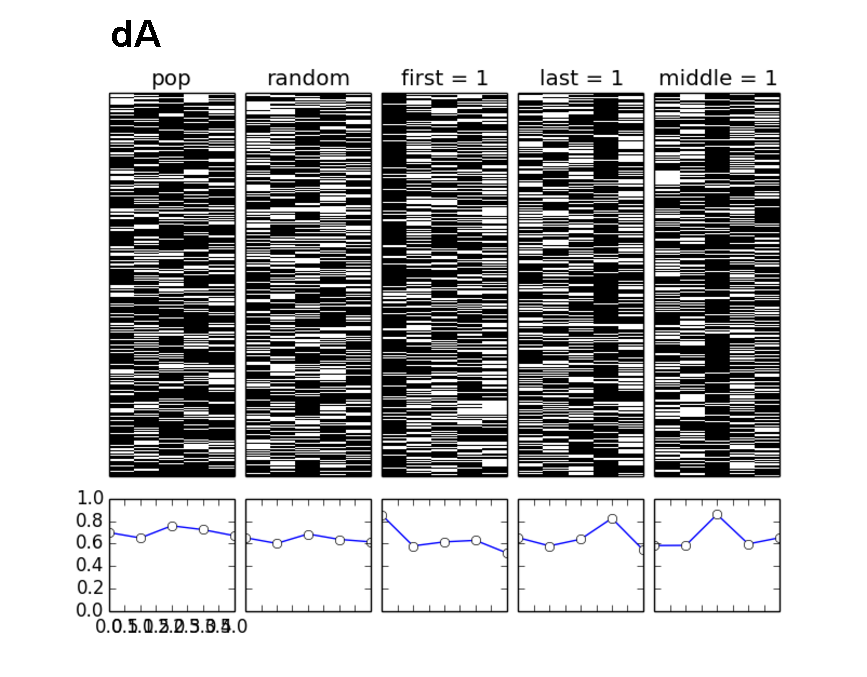
\includegraphics[scale=0.7]{da_croad.pdf}
  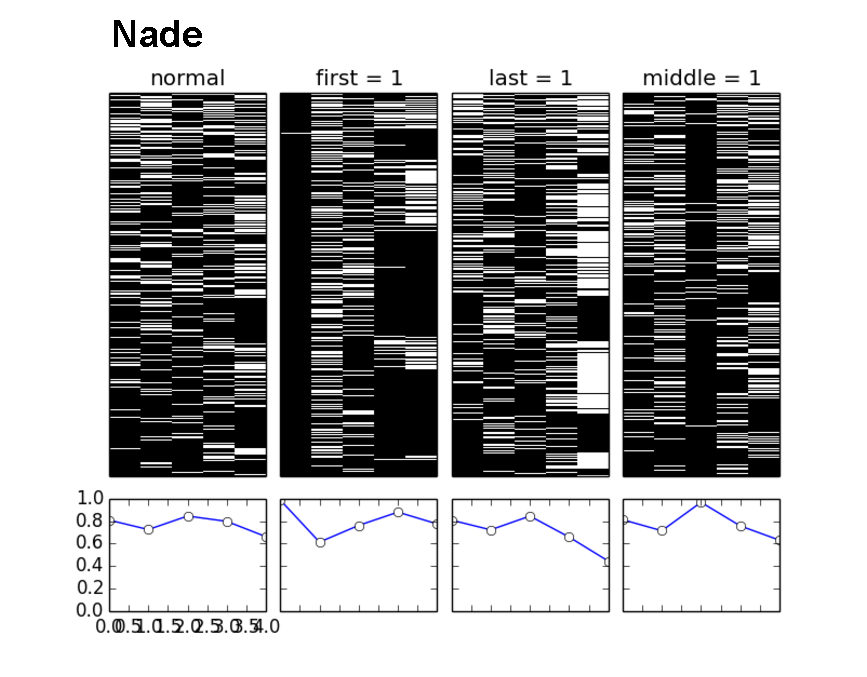
\includegraphics[scale=0.7]{nade_croad.pdf}
  \caption{}
\end{figure}

Figure 1 shows that although the algorithms have produced different distributions they have similar probabilities of solving the sub-problems. In figure 2 we now probe the models to investigate what structure has been learnt. In figure 2(a), for the dA we show the probability of solving sub-problems given different conditions. The first condition is the same as in figure 1, inputting the final population into the model. The second condition uses input from a uniform random distribution. The third, fourth and fifth also use a uniform random distribution for input but fix the sub-partitions \(\hat{p}_{1L}\) (\(c_{first}\)), \(\hat{p}_{3L}\) (\(c_{middle}\)), and \(\hat{p}_{4R}\) (\(c_{last}\)) to equal all ones, respectively. Using a random input, we see that sub-problem solutions follow a similar distribution, but the probability of solving is decreased compared to using the population. Using \(c_{first}\), there is an increase in the solutions to the first sub-problem, showing that the algorithm increases the probability of setting the sub-partition on the right to all zeroes, and suggesting that it has learnt this dependency. However, the probability of solving the long range dependency linking the first and last sub-partitions, \(\hat{p}_{1L}\) and \(\hat{p}_{4R}\), has decreased, although not drastically. Similar behaviour is seen with \(c_{last}\), where the probability of solving the sub-problem in the last partition is increased, however this leads to a small decrease in the probability of solving the long range dependency. For \(c_{middle}\) we see an increase in solving the third subproblem (which is independent from the other partitions) without any noticeable change in the probability of solving the other sub-problems.

In figure 2(b), we perform a similar probe on the NADE. Here, the first plot shows samples from the model with no bias. The second, third and fourth plots sample from the NADE but fix the probability of a 1 in the sub-partitions \(\hat{p}_{1L}\) (\(c_{first}\)), \(\hat{p}_{3L}\) (\(c_{middle}\)), and \(\hat{p}_{4R}\) (\(c_{last}\)) to be equal to 1, respectively. Differently to the dA, \(c_{first}\) with the NADE increases the probability of solving the first subproblem to almost 1, while also greatly increasing the probability of solving the long range dependency of the last sub-problem. The condition \(c_{middle}\) greatly increases the probability of solving the middle sub-problem while not greatly changing the distribution of solutions to the other sub-problems. Finally, the condition \(c_{last}\) has a negative effect, decreasing the probability of solving the last two subproblems, and affecting the long-range dependency particularly badly.

The results shown in figure 2 provide an interesting insight into the differences between the two models. The condition \(c_{first}\) provides a much greater performance increase with the NADE than with the dA. Setting the first sub-partition to all ones means that two others must be set to all zeroes. Figure 2 clearly demonstrates that the NADE is able to capture both the local and global dependency, while the dA only captures the local. However, the dA has certainly learnt complex dependencies, as in the \(c_{last}\) condition, while there is a small decrease in solving the long range dependency, it is not anywhere near as drastic as that displayed by the NADE. The dA does not suffer from ordering constraints, while the NADE does, so fixing the last sub-partition cannot influence the probabilities of the variables in earlier partitions. This implies that ordering could have a large influence on the performance of the NADE, which is a topic for further investigation. There is more flexibility in fixing inputs in the dA, which could be utilised in a hybrid search.

\begin{figure}[t!]
\centering
    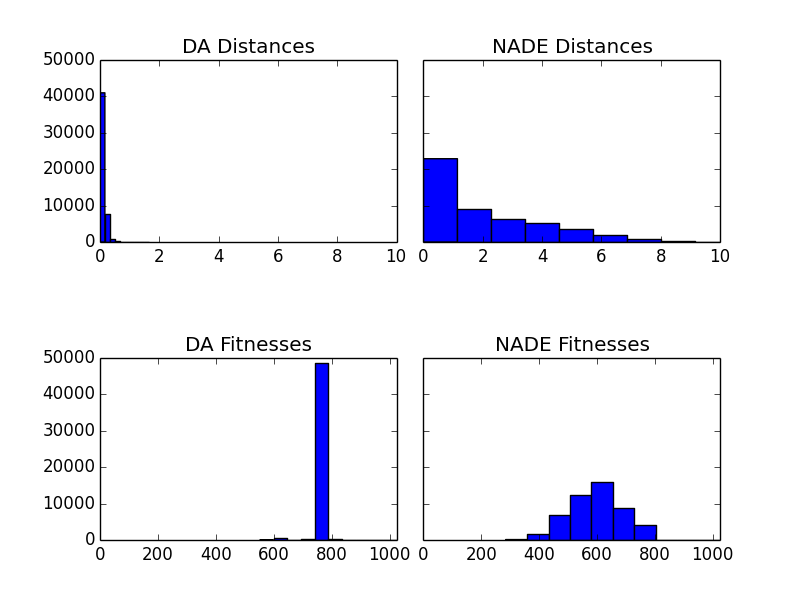
\includegraphics[scale=0.8]{hiff_hist.png}
  \caption{Hiff-128}
\end{figure}


\small

\bibliographystyle{apalike}
\bibliography{ecjsample}


\end{document}
